%opening
\title{Fourier pseudo spectral method for attenuative simulation with fractional Laplacian}

%\renewcommand{\thefootnote}{\fnsymbol{footnote}}
\author{Pengliang Yang}
%\address{ISTerre, Univ. Grenoble Alpes}

%\email{ypl.2100@gmail.com}
%\lefthead{P.L. Yang}
%\righthead{Fractional laplacian}

%\footer{SEISCOPE}


\maketitle


\begin{abstract}
This tutorial is devoted to pseudo-spectral method (PSM) by reorganizing the course material from Prof. Heiner Igel and a paper by J.M. Carcione, to illustrate how to implement viscoacoustic wave simulation based on fractional Laplacian operator. 
\end{abstract}

\section{What is a pseudo-spectral method?}


Spectral solutions to time-dependent PDEs are formulated in the frequency-wavenumber domain and solutions are obtained in terms of spectra (e.g. seismograms). This
technique is particularly interesting for geometries where partial solutions in the $\omega-k$ domain can be obtained analytically (e.g. for layered models).

In the pseudo-spectral approach - in a finite-difference like manner - the PDEs are solved pointwise in physical space $(x-t)$. However, the space derivatives are calculated using
orthogonal functions (e.g. Fourier Integrals, Chebyshev polynomials). They are either evaluated using matrix-matrix multiplications, fast Fourier transform (FFT), or convolutions.

Let us start with the 1-D acoustic wave equation.
\begin{equation}
 \frac{1}{v^2}\partial_{tt}p=\rho\partial_x\left(\frac{1}{\rho}\partial_x p\right)+f
\end{equation}
Omitting the source term, we may discretize the wave equation using standard centered finite difference for time stepping as
\begin{equation} 
\frac{p^{n+1}-2p^n+p^{n-1}}{\rho c^2\Delta t^2}=\partial_x\left(\frac{1}{\rho}\partial_x p\right)
\end{equation}
where we use the notation $p(n\Delta t):=p^n$. Thus, we have the following evolution scheme
\begin{equation}
 p^{n+1}=2p^n-p^{n-1}+\rho c^2\Delta t^2 \partial_x\left(\frac{1}{\rho}\partial_x p\right)
\end{equation}
where the space derivatives will be calculated using the Fourier transform.

\section{Computing derivatives using Fourier transform}

The Fourier transform of a function $f(x)$ and the inverse are define respectively
\begin{equation}
 \tilde{f}(\omega)=F[f]=\int f(x)e^{-i\omega x}\mathrm{d}x
\end{equation}
and 
\begin{equation}
 f(x)=F^{-1}[f]=\frac{1}{2\pi}\int \tilde{f}(\omega)e^{i\omega x}\mathrm{d}\omega
\end{equation} 
where $\tilde{f}$ is the Fourier transform of $f$. In spatial dimension, $\omega$ corresponds to the wavenumber $k$. Therefore we have
\begin{equation}
 \partial_x f=\partial_x\left( \frac{1}{2\pi}\int \tilde{f}e^{ik_x x}\mathrm{d}x\right)
= \frac{1}{2\pi}\int \underline{ik_x\tilde{f}}e^{ik_x x}\mathrm{d}x
\end{equation}
and 
\begin{equation}
 \partial_{xx} f=\partial_{xx}\left( \frac{1}{2\pi}\int \tilde{f}e^{ik_x x}\mathrm{d}x\right)
= \frac{1}{2\pi}\int \underline{(ik_x)^2\tilde{f}}e^{ik_x x}\mathrm{d}x
\end{equation}
The term $\partial_x\left(\frac{1}{\rho}\partial_x p\right)$ will be calculated by the following precedure:
\begin{equation}
\begin{array}{rl}
 p\stackrel{F}{\longrightarrow}& \tilde{p}\\
 \stackrel{ik_x}{\longrightarrow} &ik_x\tilde{p}\\
 \stackrel{F^{-1}}{\longrightarrow} &\partial_x p= F^{-1}[ik_x\tilde{p}]\\
 \stackrel{\frac{1}{\rho}}{\rightarrow} &\frac{1}{\rho}F^{-1}[ik_x\tilde{p}]\\
 \stackrel{F}{\rightarrow} & F[\frac{1}{\rho}F^{-1}[ik_x\tilde{p}]]\\
 \stackrel{ik_x}{\rightarrow} & ik_xF[\frac{1}{\rho}F^{-1}[ik_x\tilde{p}]]\\
 \stackrel{F^{-1}}{\rightarrow}& F^{-1}[ik_xF[\frac{1}{\rho}F^{-1}[ik_x\tilde{p}]]] \\
\end{array}
\end{equation}

Let us conduct a 2-D numerical simulation of acoustic wave equation with constant density. The equation is then
\begin{equation}
\partial_{tt}p=c^2 (\partial_{xx}+\partial_{zz})p
\end{equation}
Based upon Fourier transform for spatial axis, we know the right hand side of the above equation corresponds to 
\begin{equation}
-(k_x^2+k_z^2)\tilde{p}
\end{equation}
Thus, we have the following time evolution 
\begin{equation}
p^{n+1}=2p^n-p^{n-1}+\Delta t^2 c^2F^{-1}[-(k_x^2+k_z^2)F p^n]
\end{equation}

\section{Fractional Laplacian}
\inputdir{ps2d}

According to \cite{Carcione_2010_GFP}, the uniform-density pressure formulation is 
\begin{equation}
 \partial_t^2p =\omega_0^{2-2\beta} c^{2\beta} (\partial_x^2+\partial_z^2)^\beta+s
\end{equation}
where $s$ is the body force per unit; the order $\beta$ is $1\leq \beta\leq 2$. When $\beta\rightarrow 2$, it introduces stronger attenuation. Regarding the fractional order of the Laplacian operator,
we may be able to update the wavefield by
\begin{equation}
p^{n+1}=2p^n-p^{n-1}+\Delta t^2 c^2F^{-1}[(-k_x^2-k_z^2)^\beta F p^n]
\end{equation}



Another choice to perform fractional order wave simulation is
\begin{equation}
 \rho (\partial_x^\beta \rho^{-1}\partial_x^\beta +\partial_z^\beta\rho^{-1}\partial_z^\beta )
\end{equation}
which implies the following wavefield extrapolation
\begin{equation}
p^{n+1}=2p^n-p^{n-1}+\Delta t^2 c^2F^{-1}[(-1)^\beta(k_x^{2\beta}+k_z^{2\beta}) F p^n]
\end{equation}
with constant density $\rho$.

A snapshot using the code provided in the appendix is shown in Figure~\ref{fig:snapshot}, in which we use the sponge boundary condition.
% \begin{figure}
% \centering
% \includegraphics[width=0.8\textwidth]{snapshot}\\
% \caption{A snapshot of 2-D acoustic propagation using PSM method}\label{snapshot}
% \end{figure}

\plot{snapshot}{width=0.7\textwidth}{A snapshot of 2-D acoustic propagation using PSM method}


\section{Conclusion}
The Fourier method can be considered as the limit of the finite-difference
method as the length of the operator tends to the number of points along
a particular dimension.
The space derivatives are calculated in the wavenumber domain by
multiplication of the spectrum with $ik$. The inverse Fourier transform
results in an exact space derivative up to the Nyquist frequency.
The use of Fourier transform imposes some constraints on the
smoothness of the functions to be differentiated. Discontinuities lead to
Gibbs' phenomenon. As the Fourier transform requires periodicity this technique is particular useful where the physical problems are periodical (e.g. angular
derivatives in cylindrical problems).


By introducing fractional order of the Laplacian operator, we are able to perform wave simulation in attenuative medium. The computation of fractional Laplacian can be easily carried out by using Fourier pseudo spectral method, which is computational accurate and efficient enough without any additional storage when considering a constant Q model.

\appendix



\section*{Absorbing boundary condition}
\inputdir{.}
One of the easiest absorbing boundary condtion (ABC) is sponge (or referred to as Gaussian taper) boundary condition proposed by \cite{Cerjan_1985_NBC}. The principle is very simple: Attenuating the refections exponentially in the extended artificial boundary (Figure~\ref{fig:extbndr}) area by multiplying a factor less $d(u)$ than 1, i.e., $ d(u)=\mathrm{exp}(-[\alpha(nb-i)]^2), u=x,z (i\Delta x \; \mathrm{or} \; i\Delta z)$
where $nb$ is the thickness of the artificial boundary on each side of the model. A  usual choice is $\alpha=0.015$ for $nb=20\sim30$ absorbing layers. The sponge ABC can be easily applied to a wide range of wave propagation problems, including some  governing wave equations for complicated medium. 
% \begin{figure}
%   \centering
%   % Requires \usepackage{graphicx}
%   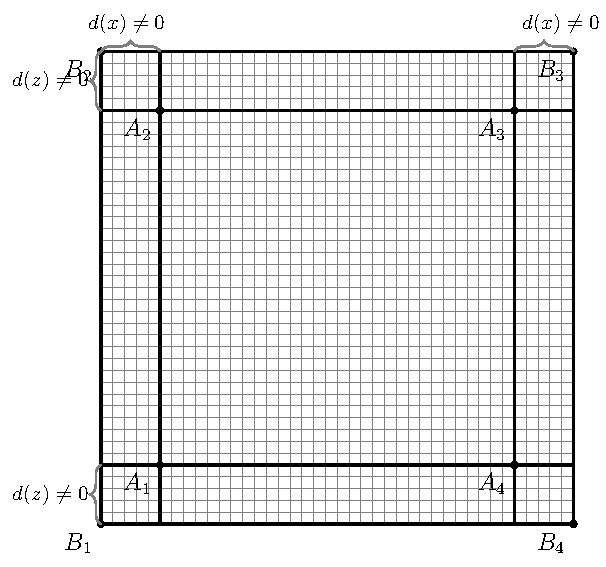
\includegraphics[width=0.6\textwidth]{extbndr}\\
%   \caption{A schematic diagram of extended artificial boundary area. $A_1A_2A_3A_4$ is the original model zone, which is extended to be $B_1B_2B_3B_4$  with artificial boundary. In the extended bounary area, the attenuation coeffcient $d(u)\neq 0$; In the model zone $A_1A_2A_3A_4$, $d(u)= 0$, $u=x,z$. }\label{fig:extbndr}
% \end{figure}

\plot{extbndr}{width=0.6\textwidth}{A schematic diagram of extended artificial boundary area. $A_1A_2A_3A_4$ is the original model zone, which is extended to be $B_1B_2B_3B_4$  with artificial boundary. In the extended bounary area, the attenuation coeffcient $d(u)\neq 0$; In the model zone $A_1A_2A_3A_4$, $d(u)= 0$, $u=x,z$.}



\bibliographystyle{plainnat}
\bibliography{fraclap}
